\chapter{COMPARISON OF LEARNING OUTCOMES FOR SIMULATION-BASED AND TRADITIONAL INFERENCE CURRICULA IN A DESIGNED EDUCATIONAL EXPERIMENT}
\label{CurriculumStudy}
 
 
\begin{center}
\textbf{Status}: Submitted for Review to \textit{Technology Innovations in Statistics Education} (TISE)\\
\end{center} 

\begin{center}
\textbf{Authors}\\
Karsten Maurer, Iowa State University, Primary Author\\
Dennis Lock, Iowa State University
\end{center}


\begin{center}
\textbf{Abstract}\\
\end{center}

Conducting inference is a cornerstone upon which the practice of statistics is based. As such, a large portion of most introductory statistics courses is focused on teaching the fundamentals of statistical inference. The goal of this study is to make a formal comparison of learning outcomes under the traditional and simulation-based inference curricula. A randomized experiment was conducted to administer the two curricula to students in an introductory statistics course.  The results indicate that students receiving the simulation-based curriculum have significantly higher learning outcomes for confidence interval related topics. While the results are not comprehensive in assessing the effect on all facets of learning, they indicate that learning outcomes for core concepts of statistical inference can be significantly improved with the simulation-based approach. 



%---------------------------------------------------------------------------
\section{Introduction}
\label{intro}

Conducting inference is a cornerstone upon which the practice of statistics is based. As such, a large portion of most introductory statistics courses is focused on teaching the fundamentals of statistical inference. In recent years the approach by which to teach inference in introductory statistics courses has been the topic of growing discussion.  The traditional approach to inference curriculum is focused on distributional theory-based methodology, often characterized by use of distributional assumptions, formulas and tables. A modern alternative is a simulation-based approach to the inference curriculum. The simulation-based approach utilizes tactile and computational simulation to run inferential techniques such as bootstrapping for confidence intervals and simulation-based hypothesis testing. Many proponents of the simulation-based inference curriculum argue that this allows students to be exposed to the core concepts of the inference without first requiring the understanding of theoretical probability distributions. 

The focus of the following study is to make a formal comparison of learning outcomes under the traditional and simulation-based inference curricula.  The learning outcomes for concepts surrounding inference with confidence intervals and hypothesis testing are of primary interest.  A randomized experiment was conducted to administer the two curricula to students in an introductory statistics course. The experimental design allows for causal inference to be drawn about the effect of curriculum type on the learning outcomes. The results indicate that significant improvement in learning outcomes for confidence interval related topics are achieved using the simulation-based teaching methods.
%---------------------------------------------------------------------------
\section{Literature Review}
\label{litreview}

With the goal to make proper comparison of traditional versus simulation-based curricula for introductory statistical courses, we must first view where each approach stands within the constant evolution of statistics education. Using the term ``traditional'' to describe the current standard for introductory statistics course curriculum is relative to only the last two decades. Moore chronicled the reform movement of statistic education of the 1980's and 1990's as a period of drastic change in the introductory statistics classroom.  The curriculum expanded greatly from a course dominated by theory-based inference methodology to the inclusion of the topics of data exploration, data production, model diagnostics and simulation.  The content change indicated a shifting emphasis toward conceptual understanding and applied statistics.  Moore also stated, ``(w)hat is striking about the current reform movement is not only its momentum but the fact that it centers on pedagogy as much as content'' \citep{Moore1997}. The pedagogical push toward active learning was combined with content change and the increasing use of technology to form what may be referred to now as the traditional introductory statistics curriculum. 

The tenets of the statistics education reform movement were formalized in the Guidelines for Assessment and Instruction in Statistics Education (GAISE) reports for pre-K-12 \citep{GAISEk12} and introductory college courses \citep{GAISEcollege}. Six recommendations were made in the executive summary of the GAISE college report: emphasize statistical literacy and thinking, use real data, stress conceptual over procedural understanding, foster active learning, use technology for both learning and analysis, and use assessment as part of the learning process.  In the past decade these principles have been widely adopted in statistics education with a noteworthy increase in technological integration.  Technology in the statistics classroom now regularly takes the form of applets, graphing calculators, multimedia materials, and educational, analytical and graphical software (\citealt{chance2007}; \citealt{Rubin2007}).  Technological proliferation in the statistics classroom came as a result of technologically receptive statistics educators taking advantage of computation that has become cheaper and more accessible.  A large survey of introductory statistics instructors found that 76\% of the instructors usually or always require students to use a computer program to explore and analyze data, and 90\% of the instructors report a high level of comfort using computer applications to teach introductory statistics \citep{Hassad2013}.  

Amidst the drastic increase in the use of technology in introductory statistics education there has been a growing group of educators who believe that the curriculum reform has stopped short of the possibilities that computation can provide.  Cobb argues that statistics education has done well to adopt technology to displace tedious calculation but has not effectively changed the approach to teaching inference.  Cobb strongly articulates a call for statistics instructors to use simulation-based methods for teaching inference to replace the traditional approach to inference using theory-based methodology.  He states, ``(o)ur curriculum is needlessly complicated because we put the normal distribution... at the center of our curriculum, instead of the core logic of inference at the center'' \citep{Cobb2007}.  If we view the introductory statistics course as a constrained optimization problem with statistical literacy and conceptual understanding of inference as the items to maximize, then removing the burden of learning the normal distribution will present the opportunity for more time spent learning core concepts \citep{Carver2011}.   In recent years, curricula for using a simulation-based approach to inference have been developed by a number of groups of statistics educators (\citealt{ISI}; \citealt{Lock5}; \citealt{CATALST};  \citealt{Carver2011}).  

There has been research done on the efficacy of simulation-based inference curricula; however, due to the recency of the curricula development most of this preliminary research has been observational.  Budgett, Pfannkuch, Regan \& Wild conduct a case study on a small group of students receiving a simulation-based curriculum and found significant learning gains using pre and post testing based on the Comprehensive Assessment of Outcomes in a First Statistics Course (CAOS).  This study does not however attempt to make a comparison between the simulation-based approach and traditional approach to teaching inference \citep{Budgett2013}. Another pair of studies make comparisons on both learning outcomes and learning retention between the two types of curricula. Tintle, VanderStoep, Holmes, Quisenberry and Swanson found weak evidence for an overall improvement in learning outcomes and significant improvements within the topic of hypothesis testing for the cohort of students receiving the simulation-based curriculum, but the lack of random assignment of student to cohort obstructs the ability to draw any causal conclusions \citep{Tintle2011}.  Tintle, Topliff, VanderStoep, Holmes and Swanson then found significant evidence for improvements to learning outcome retention after four months for students receiving the simulation-based inference curriculum, but again self-selection of students to cohort prevents establishing a causal link \citep{Tintle2012}.  

The preliminary research shows promising results for the simulation-based approach to teaching statistical inference.  A more rigorous experimental approach to comparing the traditional and simulation-based curricula has been taken in this study in order to establish a causal effect of curriculum on learning outcomes. Section 3 explains the structure and methodology implemented in the educational experiment and the measurement of student learning.  Section 4 details the model based approach for assessing the effect of curriculum on specific learning outcomes.  Lastly, we discuss the study findings and explore the implications for designing future introductory statistics curricula.
%---------------------------------------------------------------------------
\section{Methodology}
\label{methods}

The subjects for this study were students enrolled in two sections of the Introduction to Statistics, Stat 104, course at Iowa State University in the spring semester of 2014. Stat 104 is an introductory statistics course tailored for students in the agricultural and biological sciences. Of the 112 students to complete the course, 101 students consented to the release of their course data for the purposes of this study.   The students who did not consent were treated identically to those who consented, but their data was omitted from the analysis that follows.  Students from both sections were randomly assigned to one of the two inference curriculum treatments, creating cohorts A,C and B,D, respectively. Cohorts A and B were exposed to the simulation-based curriculum; while the cohorts C and D were exposed to the traditional curriculum. Student cohorts were the basic units to which room assignments, instruction and curriculum treatments were applied.

The course was administered by the authors in a co-teaching setting for students from all cohorts. The course schedule involved two hours of lecture and two hours of lab per week.  The co-teaching strategy was employed as an intentional attribute of the experimental design. The following subsections will detail the curriculum outline for each cohort of students, the experimental design for administering the curricula using the strengths of the co-teaching setup and the data collected for analysis.
%-----------------------------------------------------
\subsection{Curricula Structures}
\label{curric}

To compare the learning outcomes for students receiving the traditional and simulation-based inference curricula we first needed to prepare a curriculum for each approach.  Both curricula needed to satisfy the course guidelines set by the Department of Statistics at Iowa State University, covering the following topics: univariate and bivariate descriptive statistics, linear regression, experimental design, basic probability rules, the binomial distribution, the normal distribution, sampling distributions, and inference on means and proportions. Each curriculum was composed of lecture, corresponding lecture notes, weekly lab assignments designed for groups of four to five students, weekly homework assignments, a midterm exam and a cumulative final exam.  The curricula materials for the course did not require the use of a textbook, however specific textbooks that roughly follow the structure of each curriculum were recommended as supplementary study materials (\citealt{AgrestiFranklin}; \citealt{Lock5}).

Figure~\ref{fig:CurricSched} outlines how these topics were structured within a weekly schedule for the sixteen week semester for each curriculum.  Note that students from all cohorts were exposed to an identical curriculum for all non-inference related topics in the course. This includes identical lecture, course notes, homework assignments, lab assignments and midterm exam during the first half of the semester.

Starting at week 9 the curricula diverge into their respective approaches to inference.  Cohorts A and B began the simulation-based inference curriculum in week 9 by first learning the concepts of sampling distributions then used computer simulation and sampling variability as a basis for exploring inference using bootstrap confidence intervals and simulation-based tests.  To be specific, confidence intervals were constructed by estimating the standard error using the standard deviation of the bootstrap distribution, not through percentile-based bootstrap methods.  Lectures, homework and labs for these cohorts utilized the StatKey software package \citep{Lock5} to conduct the simulation-based inference. The simulation-based curriculum then covered normal distributions and how they could be used to conduct inference on means and proportion.  While many advocates for simulation-based methods may argue that the normal distribution should be pushed to a second course in statistics, course guidelines required that all students of this introductory statistics course be taught theory-based inference methodology.  

\begin{figure}[hbtp]
\centering
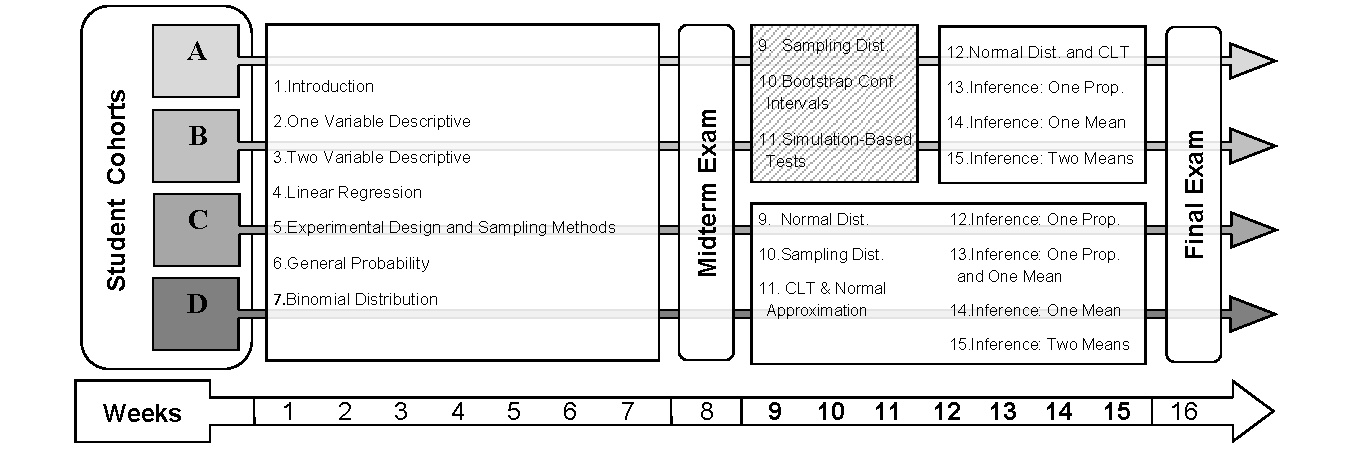
\includegraphics[keepaspectratio=true, width=1\textwidth]{CurriculumStudy/CurriculaPaths2.pdf}
\caption{\label{fig:CurricSched} Curricula Schedules}
\end{figure}

Cohorts C and D progressed through the traditional approach by first learning the normal distribution and use of the normal tables. They were then introduced to applications of the normal approximation within inference.  The traditional curriculum utilized simulation to display concepts, but only to the extent of demonstrating that sampling distributions can be approximated by normal distributions under certain conditions.  

During the second half of the semester the lectures, course note, homework and lab assignments differed between the two curricula.  However, homework and lab assignments were kept similar when they covered similar topics.  For example, all cohorts covered the topic of sampling distributions so the lab assignments were nearly identical between the two groups with the exception of a question pertaining to the normal approximation included for the traditional cohorts.  By the end of the semester all cohorts covered how to conduct inference using normal theory; however cohorts A and B additionally learned the core concepts of inference using simulation-based methods prior to learning traditional theory-based inference methods.  

%-----------------------------------------------------
\subsection{Experimental Design}
\label{design}

The logistics of administering a course with two distinct curricula and four cohorts of students required a well-structured design and creative scheduling on several fronts.  The primary objectives for the experimental design were to eliminate differences in non-inference related curriculum administration to the extent possible, remove the confounding instructor effect on each curriculum and to mitigate the effect of unknown lurking variables through random assignment of students to curricula.  

Students were randomly assigned to cohorts during the first week of the course.  Of the 101 students who completed the course and consented to the release of their data there were 50 students in the traditional treatment group and 51 students in the simulation-based treatment group. It is also worthwhile to note that of the 4 students to drop the course, all did so prior to week 9; thus, we can safely assume that the inference curriculum treatment did not play a role in the drop. All students who began the inference curricula completed the course.

Students were exposed to identical lecture and lab instruction for the first half of the semester and then diverge into two separate lecture and lab settings for the second half of the semester. This was done to make the experience as similar as possible such that both treatment groups would have the same exposure to terminology and ideas leading up to the inference topics. We could not reassign students to lecture and lab times different than the times for which they enrolled, which meant the logistics of the design required preemptive room scheduling and course time scheduling preparations.  By working with the department chair and course coordinator before students enrolled into sections, we were able to schedule two sections of the course to have identical lecture times but separate lab times. Special room scheduling was required because all students needed to attend the same lecture and lab rooms for the first half of the semester then split into separate lecture and lab rooms after the midterm.  This room and course time scheduling allowed for students to be divided into cohorts and attend the lecture or lab specific to their curriculum.  The lecture and lab room schedules for each cohort are displayed in Figure~\ref{fig:InstSched}.

\begin{figure}[hbtp]
\centering
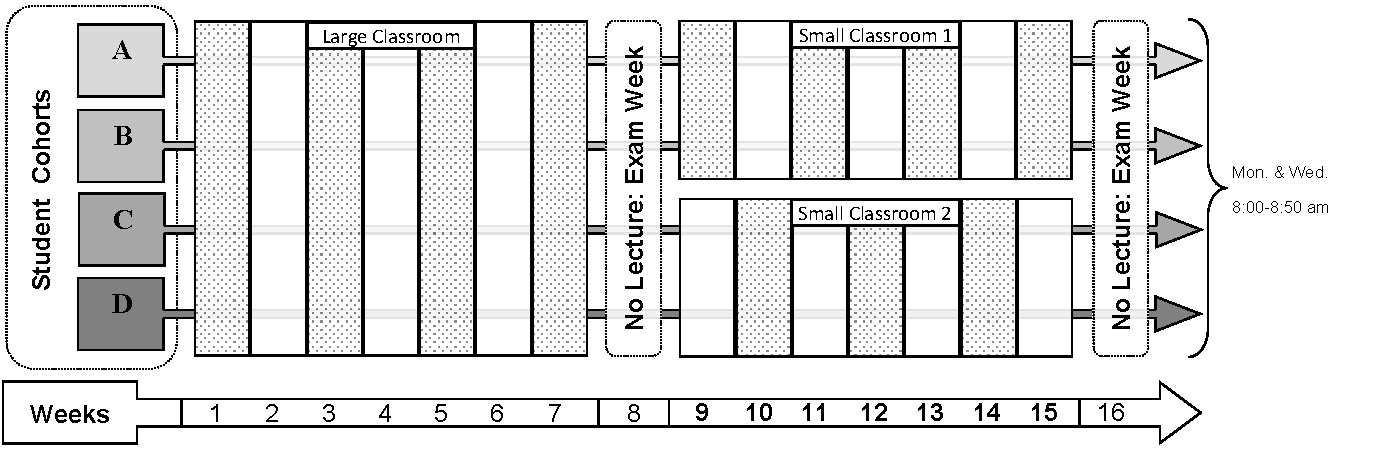
\includegraphics[keepaspectratio=true, width=1\textwidth]{CurriculumStudy/LectureInstructionWithRooms.pdf}\\
\vspace{.5cm}
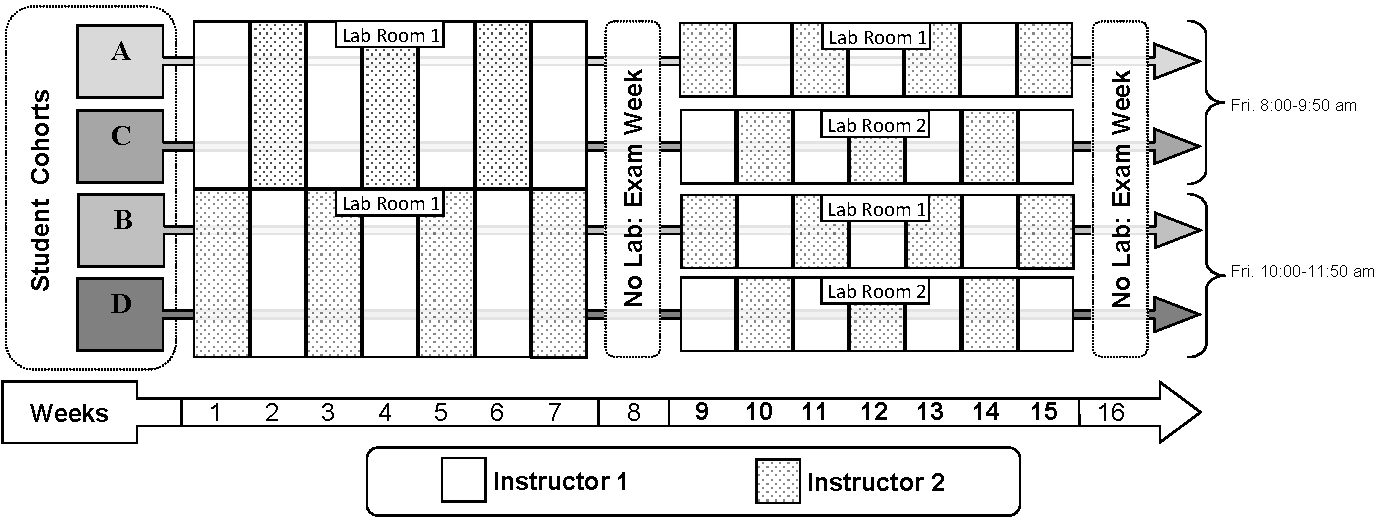
\includegraphics[keepaspectratio=true, width=1\textwidth]{CurriculumStudy/LabInstructionWithRooms.pdf}
\caption{\label{fig:InstSched} Instructor and Room Schedule}
\end{figure}


Assigning one instructor to each curriculum would confound the instructor effect and the curriculum effect.  To avoid confounding, each treatment group would need to receive instruction from both instructors.  An alternating weekly schedule was decided upon to spread out the instructor effects over both curricula. A coin was flipped to decide how to match the instructor to the curriculum when the alternation was initialized. The lecture and lab instruction schedules for each cohort can also be found below in Figure~\ref{fig:InstSched}. Note that each figure has student cohort and times fixed across all weeks, reflecting the unchanged time structure that each student enrolled into. The instructors and room locations are what changed throughout the course. 

%-----------------------------------------------------
\subsection{Data Collection}
\label{datacollect}

In order to measure learning outcomes for specific inference concepts we utilized question sets from the Assessment Resource Tools for Improving Statistical Thinking (ARTIST) for the topics of confidence intervals and hypothesis testing \citep{ARTIST}.  The ARTIST scaled question sets each consist of 10 multiple choice questions that are geared toward critical thinking about the inference topic.  These questions were administered as part of the written final exam for all students on the same day and time. The ARTIST scaled scores for the topics of confidence interval and hypothesis testing were recorded for each student. The multiple choice questions for the ARTIST scaled topics can be found in Appendix~\ref{appendA}.

The final exam also included two problems that tested the student's ability to conduct statistical inference in an applied setting using theory-based methodology. Each problem was based on a hypothetical scenario where data has been collected and inference needed to be conducted using the traditional approach using formulas and tables. The first problem provided data summaries and students needed to construct and interpret a confidence interval for a single population mean. The second problem required students to conduct a hypothesis test for a single proportion based on another set of data summaries. The applied inference problem scores for each student are not used for the primary analysis on learning outcomes but are included for an interesting peripheral analysis on student ability to conduct inference using traditional theory-based methods. The applied inference problems and grading rubrics can also be found in Appendix~\ref{appendA}. The exams were graded blindly, with no identifying information of the student or treatment visible during the grading process.

In addition to the ARTIST and applied inference question scores, data were collected from the first eight weeks of the course -- prior to student exposure to an inference curriculum. We have scores from homework assignments 1 to 7, lab assignments 1 to 7 and the midterm exam for each student. The midterm exam questions and grading rubrics can be found in Appendix~\ref{appMidtermExamQuestions}. Since all of these items were administered and graded equivalently for all students before being assigned to a curricula, the scores from these weeks will be referred to as the ``pre-treatment measurements''. Lastly, the data include the cohort to which each student belonged.

The research proposal approved by the Institutional Review Board specified that students' data would be entirely deidentified following the course, including all demographic information.  At the conclusion of the semester the data for the 101 students who consented to the release of their data were saved, with names and identity information removed, to a spreadsheet.  The deidentified student data was imported to \texttt{R} for the analysis described in Section~\ref{analysis} below. 


%-----------------------------------------------------
\subsection{Data Summary}
\label{dataSummary}

The ARTIST and applied inference question scores from the final exam are the response variables on which we wish to compare the groups of students from the two inference curricula. Figure~\ref{fig:ScoreHistsByGroup} displays the histogram, mean and standard deviation for each response variable, separated by curricula.  Midterm exam scores as also included in order to provide a comparison of the curricula groups using a pre-treatment measurement. 

\begin{knitrout}
\definecolor{shadecolor}{rgb}{0.969, 0.969, 0.969}\color{fgcolor}\begin{figure}[H]

{\centering 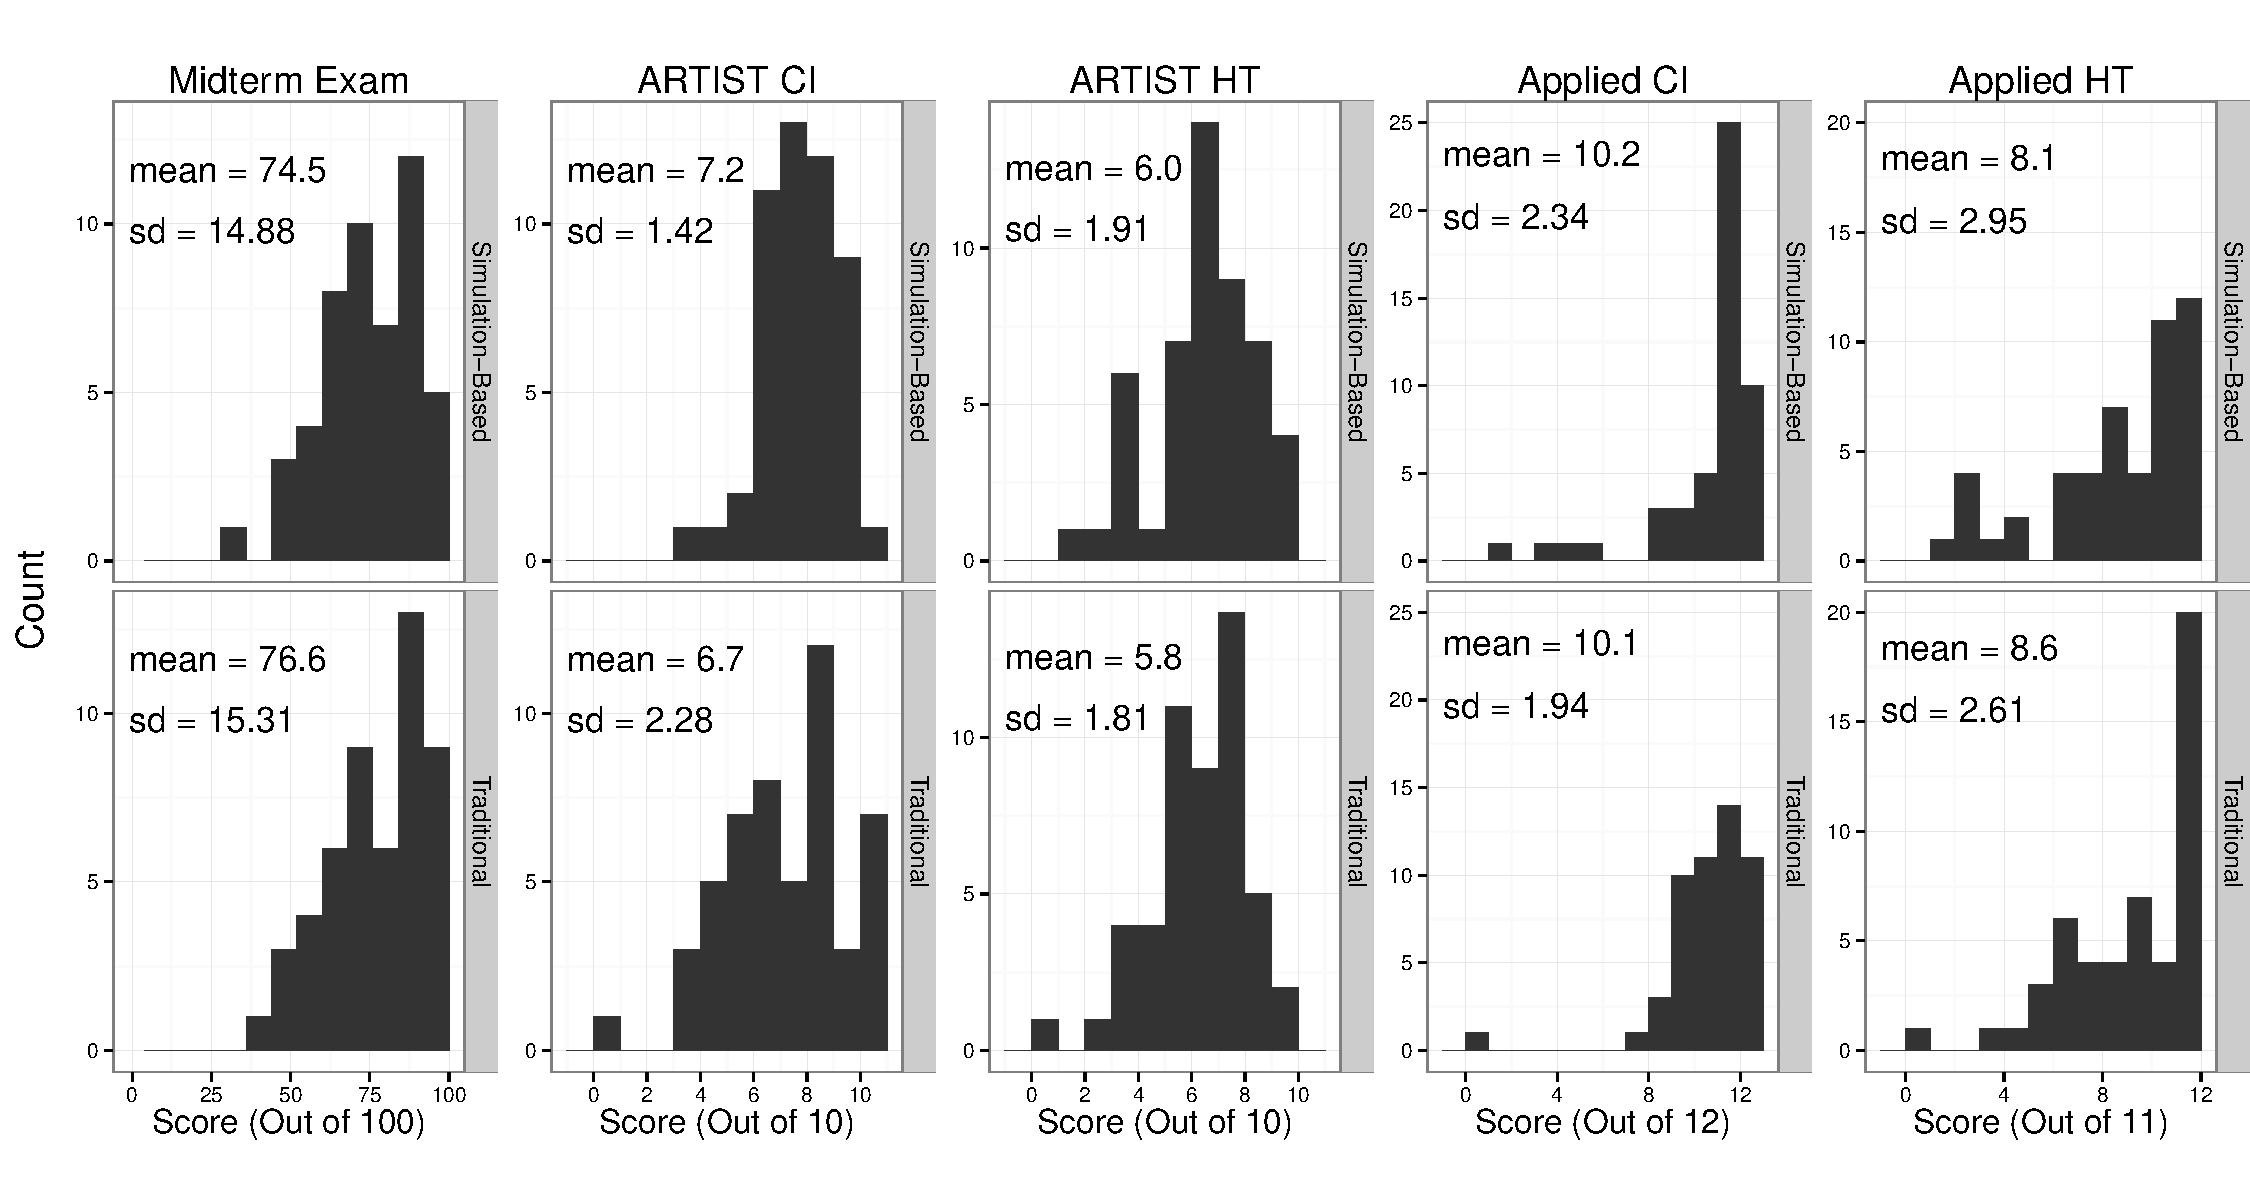
\includegraphics[width=1\linewidth]{figure/ScoreHistsByGroup-1} 

}

\caption[Histograms and summary statistics of scores separated by curricula group]{Histograms and summary statistics of scores separated by curricula group.}\label{fig:ScoreHistsByGroup}
\end{figure}


\end{knitrout}
\vspace{.05in}
In Figure~\ref{fig:ScoreHistsByGroup}, we see that the midterm exam scores are very similarly distributed for each group; with the traditional curriculum group scoring only slightly higher on average than the simulation-based curriculum group. This similarity is expected -- and desirable -- because the midterm was conducted prior to the treatment being administered, and the class materials and instruction were designed to be identical at that stage of the course.

Comparing the distributions in Figure~\ref{fig:ScoreHistsByGroup} we see that the simulation-based inference group had a higher average score than the traditional inference group on both of the ARTIST scaled question sets and on the applied confidence interval problem, but scored lower on average on the applied hypothesis testing problem.  The simulation-based inference group had lower variability than the traditional inference group on the ARTIST question set for confidence intervals, but higher variability on all other scores. These data summaries are suggestive of differences in the inference learning outcomes of the two groups. In Section~\ref{analysis}, we take a model-based approach to assess if these differences are statistically significant.




% 
% % latex table generated in R 3.0.2 by xtable 1.7-3 package
% % Mon Nov 24 15:50:03 2014
% 
% \begin{table}[ht]
% \small
% \centering
% \begin{tabular}{llrrrrr}
%   \hline
%     & Curriculum & Midterm & ARTIST CI & ARTIST HT & Applied CI & Applied HT \\ 
%   \hline
%   & Traditional & roomdat[1,3] & roomdat[1,4] & roomdat[1,5] & roomdat[1,6] & roomdat[1,7] \\ 
%    & Simulation & roomdat[2,3] & roomdat[2,4] & roomdat[2,5] & roomdat[2,6] & roomdat[2,7] \\ 
%  \hline
%  & & & & & &  \\ 
%  & & & & & &  \\ 
%  \hline
%   
%  Midterm Quartile & Curriculum & Midterm & ARTIST CI & ARTIST HT & Applied CI & Applied HT \\ 
%   \hline
% 1st Quartile & Traditional & 55.50 & 55.38 & 56.92 & 81.41 & 61.54 \\ 
%  & Simulation & 55.68 & 64.29 & 50.00 & 74.40 & 62.34 \\ 
%  & Difference & -0.18 & -8.90 & 6.92 & 7.01 & -0.80 \\ 
%  \hline
% 2nd Quartile & Traditional & 73.19 & 57.69 & 51.54 & 77.56 & 69.23 \\ 
%  & Simulation & 71.00 & 71.67 & 52.50 & 86.11 & 66.67 \\ 
%  & Difference & 2.19 & -13.97 & -0.96 & -8.55 & 2.56 \\ 
%  \hline
% 3rd Quartile & Traditional & 84.58 & 76.15 & 57.69 & 88.46 & 90.91 \\ 
%  & Simulation & 82.71 & 71.67 & 61.67 & 84.72 & 75.00 \\ 
%  & Difference & 1.87 & 4.49 & -3.97 & 3.74 & 15.91 \\ 
%  \hline
% 4th Quartile & Traditional & 94.33 & 78.33 & 65.83 & 90.97 & 93.94 \\ 
%  & Simulation & 91.67 & 82.50 & 76.67 & 95.83 & 93.18 \\ 
%  & Difference & 2.67 & -4.17 & -10.83 & -4.86 & 0.76 \\ 
%    \hline
% \end{tabular}
% \caption{Average percentage scores broken down by midterm exam quartiles.}
% \label{tab:examquartiles}
% \normalsize
% \end{table}



%---------------------------------------------------------------------------
\section{Analysis}
\label{analysis}

The primary goal of the analysis is to investigate if there is a curricula effect on inference concept learning outcomes.  Our data includes ARTIST scaled topic scores for confidence intervals and hypothesis tests which we use as the responses for the comparison of curricula. A model based approach is used to assess curricula effect while controlling for pre-treatment differences between students. With the two dimensional response and an assortment of covariates we employ a multivariate analysis of covariance (MANCOVA) model.   

Both curricula groups were required to learn how to conduct normal-based inference. This leads to another question of interest. Does the added simulation-based material turn out to be detrimental to student's ability to use distributional theory-based methods to conduct inference?  Two applied problems were included on the final exam that required students to use theory-based methods and formulas to conduct inference. These applied questions were used as the responses in a separate MANCOVA model to check for a curriculum effect. 

The bivariate MANCOVA models used for these two analyses are parameterized as 

\begin{eqnarray}\label{eq:mancova}
y_{i\ell} = \tau_{\ell} \mathbbm{1}_{\{i \in T\}} + \beta_{\ell 0} + \sum_{p=1}^{P}x_{ip}\beta_{\ell p} + \epsilon_{i\ell},
\end{eqnarray}
where 

\begin{tabular}{lp{5in}}
$y_{i\ell}$ &  is the $\ell^{th}$ response ($\ell \in \left\{1,2\right\}$) from  student $i$, $ 1 \le i \le n$,\\
$\tau_{\ell}$ & is the treatment effect of the simulation-based curriculum on response $\ell$, and \\
$\mathbbm{1}_{\{i \in T\}}$ & is an indicator function, that is one, if student $i$ is in the treatment group, and zero otherwise.\\
$\beta_{\ell 0}$ & is the common intercept for response $\ell$, and \\
$\beta_{\ell p}$, & $1 \le p \le P$ are the model coefficients of the $P$ covariates. \\
$x_{ip}$ & is the $p^{th}$ pre-treatment covariate score of student $i$, and\\
$\epsilon}_{i\ell}$ & is the error for the $\ell ^{th}$ response from the $i^{th}$ student. 
\end{tabular}

We assume that error pairs are independent and identically distributed:
\[
\vec{\epsilon}_{i} = 
\begin{bmatrix}
  \epsilon_{i1} \\ \epsilon_{i2} 
 \end{bmatrix}  
 \distas{iid} \text{MVN} \left( 
 \begin{bmatrix}
  0 \\ 0 
 \end{bmatrix},
 \Sigma = \begin{bmatrix}
  \sigma_{11}^2 & \sigma_{12}^2 \\ 
  \sigma_{21}^2 & \sigma_{22}^2
 \end{bmatrix}
 \right)
\]

% \begin{center}
% $y_{ik} = \tau_{k} \mathbbm{1}_{\{i \in T\}} + \beta_{0k} + \Bigg(\sum_{p=1}^{P}x_{ip}\beta_{pk}\Bigg) + \epsilon_{ik}$,\\
% 
% where $k \in \left\{1,2\right\}$,  $i \in \left\{1,...,n\right\}$, and $p \in \left\{1,...,P\right\}$,
% 
% $\vec{\epsilon}_{i} = 
% \begin{bmatrix}
%   \epsilon_{i1} \\ \epsilon_{i2} 
%  \end{bmatrix}  
%  \distas{iid} $ MVN$\left( 
%  \begin{bmatrix}
%   0 \\ 0 
%  \end{bmatrix},
%   \begin{bmatrix}
%   \sigma_{11}^2 & \sigma_{12}^2 \\ 
%   \sigma_{21}^2 & \sigma_{22}^2
%  \end{bmatrix}
%  \right)$,
% \end{center}

With this parameterization, it is clear that the underlying structure of the MANCOVA model is a multivariate multiple linear regression that can include categorical and continuous covariates. Note that the paired error terms from each student are correlated but are specified as independent between students. The assumption of independence between student response scores is understood to be unrealistic for students from the same class. \km{The repercussions of violating the assumption of independence between student responses will be explored through a simulation study in Section~\ref{SimStudy} following the analysis.}

%-----------------------------------------------------
\subsection{Modeling ARTIST Outcomes}
\label{ArtistModel}

We begin with the model for the ARTIST scaled topic scores.  Many of the pre-treatment variables are highly correlated. To select a model with only the most predictive pre-treatment covariates, model selection was conducted by first running backward selection based on AIC then removing further covariates that posed collinearity issues. The model selected for final analysis included three covariates: an indicator variable for the curriculum treatment group, the lab 5 score and the midterm score.  The midterm tested students on materials from weeks 1-7 and lab 5 assessed understanding of topics related to random selection techniques.  We will refer to this selected model as the ``ARTIST Model''. Model fit for the ARTIST Model was assessed to be satisfactory; see Appendix~\ref{appARTISTModDiag} for residual plots and other model diagnostics.





To test for overall covariate effects on the multivariate responses we use Pillai's $\Lambda$. Table~\ref{tab:overallmod} shows a weak overall effect of the curriculum treatment on the paired ARTIST scaled topic scores.  This prompts us to investigate the treatment effect on the ARTIST scaled topic scores for confidence intervals and hypothesis tests separately, to see if the weak overall effect is driven by a significant effect on one of the two scores.

\begin{table}[hbtp]
\centering
\begin{tabular}{lrrr} \hline
 & Pillai's $\Lambda$ & Approx. F & Pr($>$$|$F$|$)\\ 
 \hline  
Midterm & 0.2109 & 12.8277 &
0.0000\\ 
Lab 5 & 0.0792 & 4.1261 &
0.0191\\ 
Treatment & 0.0469 & 2.3605 &
0.0998\\ 
\hline
\end{tabular}
\caption{Tests for overall covariate effects on ARTIST question scores using Pillai's $\Lambda$.}
\label{tab:overallmod}
\end{table}

To investigate the effect of the curriculum treatment on each ARTIST scaled topic score, we analyze the two underlying linear models that comprise the overall MANCOVA model. Table~\ref{tab:cimod} displays the coefficients of the linear model fit to the ARTIST scaled score for confidence interval learning outcomes along with covariate ranges to provide context to coefficient magnitudes. It should be noted that although the midterm and lab scores were recorded discretely, they were treated as continuous covariates when fitting the model. We find that midterm, lab 5 and the curriculum treatment effect are significant. Specifically, the simulation-based inference group scored significantly higher by 0.7149 out of a possible 10 points, a 7.146\% improvement in confidence interval learning outcomes on the ARTIST scale while controlling for midterm and lab 5 scores.\\


% latex table generated in R 3.0.2 by xtable 1.7-3 package
% Tue Jul 29 15:46:21 2014
\begin{table}[hbtp]
\centering
\begin{tabular}{rccc}
  \hline
 & Covariate Values & Estimate & 95\% Confidence Interval \\ 
  \hline
Intercept & 1 & 1.4648 & ( -0.5467 , 3.4763 ) \\ 
  Midterm & \{0,1,...100\} & 0.0477 & (  0.0253 , 0.0701 ) \\ 
  Lab 5  &  \{0,1,...100\} & 0.0183 & (  0.0057 , 0.0309 ) \\ 
  Treatment &  \{0,1\} & 0.7146 & (  0.0435 , 1.3858 ) \\ 
   \hline
\end{tabular}
\caption{Coefficients for model fit to ARTIST score for confidence interval topic.}
\label{tab:cimod}
\end{table}

Table~\ref{tab:htmod} displays the coefficients of the linear model fit to the ARTIST scaled score for hypothesis test learning outcomes.  We find that only the midterm score is significant for predicting learning outcomes for hypothesis testing. There was no significant curriculum treatment effect. \\

% latex table generated in R 3.0.2 by xtable 1.7-3 package
% Tue Jul 29 15:41:44 2014
\begin{table}[hbtp]
\centering
\begin{tabular}{rccc}
  \hline
 & Covariate Values & Estimate & 95\% Confidence Interval \\ 
  \hline
Intercept & 1 & 2.1053 & ( 0.0046 , 4.2060 ) \\ 
  Midterm & \{0,1,...100\} & 0.0386 & (  0.0152 , 0.0620 ) \\ 
  Lab 5  &  \{0,1,...100\} & 0.0085 & (  -0.0046 , 0.0217 ) \\ 
  Treatment &  \{0,1\} & 0.3050 & (  -0.3960 , 1.0059 ) \\ 
   \hline
\end{tabular}
\caption{Coefficients for model fit to ARTIST score for hypothesis test topic.}
\label{tab:htmod}
\end{table}



A final consideration in the comparison of learning outcomes using the ARTIST model is that we made two primary comparisons; the curriculum effect on each of the inference topics. While several multiple comparisons adjustments have been developed for univariate response modeling, the Bonferroni method is the only traditional adjustment that is flexible enough for use in the MANCOVA setting. With the Bonferroni adjustment, if we wish to maintain an overall $\alpha=0.05$ significance level then we hold each individual comparison to the $\alpha=0.025$ level. After using the Bonferroni adjustment, the curriculum effect on learning outcomes for confidence interval topics would no longer considered significant ($\text{p-value} = 0.031 > 0.025$) at the overall $\alpha = 0.05$ level, but instead would be significant at the overall $\alpha = 0.1$ level.  However, the Bonferroni method is well known for being overly conservative in its adjustment, and we are comfortable with maintaining the original interpretations.

%-----------------------------------------------------
\subsection{Modeling Applied Theory-Based Inference Scores}
\label{AppliedModel}

As with the MANCOVA model for ARTIST scaled question scores, we consider all pre-treatment measurements in a new model for the two applied theory-based inference question scores.  Backward stepwise selection was used to obtain a reduced MANCOVA model in a model selection process identical to that described in Subsection~\ref{ArtistModel}. We will refer to the selected model here as the ``Applied Model''.  Residual plots and other model diagnostics for the Applied Model may be found in Appendix~\ref{appAppliedModDiag}.

Table~\ref{tab:overallmod1} shows -- based the Pillai's $\Lambda$ -- that there was no overall effect of curriculum treatment on the scores for the pair of applied inference problems. This is of particular interest because students receiving the simulation-based curriculum had three weeks less of coursework involving the use of normal distributions and normal tables. This implies that despite the increased complexity of the simulation-based material and the shortened exposure to theory-based inference concepts, there was no significant detriment to students' performance in conducting inference using theory-based methods. It should be noted that the applied questions from the final exam were written by the authors and have not been assessed as reliable metrics for learning outcomes. Thus, the results are reported as supplementary to the discussion on learning outcomes measured by the ARTIST scaled topics.



\begin{table}[hbtp]
\centering
\begin{tabular}{lrrr} \hline
 & Pillai's $\Lambda$ & Approx. F & Pr($>$$|$F$|$)\\ 
 \hline  
Midterm & 0.3238 & 22.9881 &
0.0000\\ 
Homework 2 & 0.0870 & 4.5750 &
0.0127\\ 
Treatment & 0.0108 & 0.5217 &
0.5952\\ 
%Treatment & round(summarytab1[4,2],4) & round(summarytab1[4,3],4) &
%round(summarytab1[4,6],6)\\ 
\hline
\end{tabular}
\caption{Tests for overall covariate effects on Applied question scores using Pillai's $\Lambda$.}
\label{tab:overallmod1}

\end{table}



\km{
%-----------------------------------------------------
\subsection{Model Assessment}
\label{SimStudy}

The bivariate MANCOVA models that were employed in Sections~\ref{ArtistModel}~and~\ref{AppliedModel} make the assumption of independent errors between students; an assumption which is very likely violated in practice because learning outcomes for students attending the same lectures and labs are very likely related. The assumption of independence is typically made for convenience. The lack of repetition on the lecture and lab levels prevents us from estimating a proper variance structure. It is therefore important to assess the consequences of this violation on the fitted MANCOVA model; specifically, the impact on the Type 1 error rates in tests for curriculum effects on learning outcomes. We elect to explore the consequences through a simulation study wherein the assumption of independence is knowingly violated and the effects on errors rates can be recorded.}

\km{We choose the ARTIST Model (\ref{eq:mancova}) from Sections~\ref{ArtistModel} as the basis for our simulation study. Under the assumption of independence between students, we found weak evidence of a curriculum effect on the bivariate ARTIST learning outcomes using Pillai's test. Further inspection of the individual responses using t-tests revealed significant evidence of a curriculum effect on confidence interval learning outcomes, but no evidence of a curriculum effect on hypothesis test learning outcomes. In order to assess the trustworthiness of the results, we must first know how a violation of the assumption of independence impacts the Type 1 error rates for these tests. We simulate responses from a generative model without a curriculum effect on learning outcomes (i.e.\ $\tau_{1} = \tau_{2} = 0$) and where the assumption of independence between students is violated to a known degree. We then track the Type 1 error rate in curriculum effects when the ARTIST model, assuming independence, is fit to the simulated responses.}

\km{The generative model for the simulations is adapted from the MANCOVA model~(\ref{eq:mancova}) by adding random effects to violate the independence between students. The generative model includes fixed effects for lab 5 and midterm scores, and random effects for student responses, lab sections and lecture section. Recall that responses are nested within students, students are nested within lab sections, and labs are nested within lecture sections. Thus the generative model is defined as,
%
\begin{eqnarray}\label{eq:simgenerative}
y_{ijk\ell} = \left[ \beta_{0k} + x_{ijk1}\beta_{k1} + x_{ijk2}\beta_{k2} \right] + \left[ \eta_{\ell} + \gamma_{k\ell} + \delta_{jk\ell} + \epsilon_{ijk\ell} \right],
\end{eqnarray}
%
for $i \in \left\{1,\dots,n\right\}$, $j \in \left\{1,2,3,4\right\}$, $k \in \left\{1,2\right\}$, and $\ell \in \left\{1,2\right\}$.  Where $y_{ijkl}$ is the $\ell^{th}$ response from student $i$ who is in lab section $j$ and lecture section $k$. The fixed effects portion of the model, within the first square brackets, is defined identically to the original ARTIST model~(\ref{eq:mancova}). In the generative model the $\beta$ coefficients are set equal to the corresponding coefficient estimates from the original ARTIST model. The remaining terms, $\eta_{\ell}$, $\gamma_{k\ell}$, $\delta_{jk\ell}$, and $\epsilon_{ijk\ell}$ are random effects for ARTIST topics, lecture sections, lab sections and individual errors, respectively. These random effects are defined as
%
\[
\vec{\epsilon}_{ijk} = 
\begin{bmatrix}
  \epsilon_{ijk1} \\ \epsilon_{ijk2} 
 \end{bmatrix}  
 \distas{iid} \text{MVN} \left( 
 \begin{bmatrix}
  0 \\ 0 
 \end{bmatrix},
 \Sigma = \begin{bmatrix}
  \sigma_{11}^2 & \sigma_{12}^2 \\ 
  \sigma_{21}^2 & \sigma_{22}^2
 \end{bmatrix} 
 \right),
\]
\[
\vec{\delta}_{jk} = 
\begin{bmatrix}
  \delta_{jk1} \\ \delta_{jk2} 
 \end{bmatrix}  
 \distas{iid} \text{MVN} \left( 
 \begin{bmatrix}
  0 \\ 0 
 \end{bmatrix},
 d\Sigma = \begin{bmatrix}
  d\sigma_{11}^2 & d\sigma_{12}^2 \\ 
  d\sigma_{21}^2 & d\sigma_{22}^2
 \end{bmatrix} 
 \right),
\]
\[
\vec{\gamma}_{k} = 
\begin{bmatrix}
  \gamma_{k1} \\ \gamma_{k2} 
 \end{bmatrix}  
 \distas{iid} \text{MVN} \left( 
 \begin{bmatrix}
  0 \\ 0 
 \end{bmatrix},
 g\Sigma = \begin{bmatrix}
  g\sigma_{11}^2 & g\sigma_{12}^2 \\ 
  g\sigma_{21}^2 & g\sigma_{22}^2
 \end{bmatrix} 
 \right),
\]
\[
\vec{\eta} = 
\begin{bmatrix}
  \eta_{1} \\ \eta_{2} 
 \end{bmatrix}  
 \distas{iid} \text{MVN} \left( 
 \begin{bmatrix}
  0 \\ 0 
 \end{bmatrix},
 z\Sigma = \begin{bmatrix}
  z\sigma_{11}^2 & z\sigma_{12}^2 \\ 
  z\sigma_{21}^2 & z\sigma_{22}^2
 \end{bmatrix} 
 \right).
\]

Thus the variance structure for the responses includes common variance components $\sigma_{\ell\ell'}$ and scaling parameters $z$, $g$ and $d$. The variance estimates for $\sigma_{\ell\ell'}$ from the original ARTIST model are plugged in as variance parameters for the generative model. The scaling parameter $z$ controls the variability that is common between all student responses; thus $z \sigma_{\ell\ell'}$ is the covariance of responses for ARTIST sets $\ell$ and $\ell'$ between students that do not share lecture or lab sections. The scaling parameter $g$ controls the additive increase to covariance between students of the same lecture section, $g \sigma_{\ell\ell'}$, and $d$ controls the additive increase to covariance between students of the same lab section, $d \sigma_{\ell\ell'}$. If each of these variance scaling parameters is set to zero, there is no violation to the assumption of independence between students; thus making the variance structure of the generative model~(\ref{eq:simgenerative}) match the error structure of the original ARTIST model~(\ref{eq:mancova}). However, these parameters may be adjusted to violate the independence assumption to different degrees.}

\km{The simulation procedure for assessing the Type 1 error rates under violations of independence between student responses is conducted through a five step process. We consider violations based on all combinations of $d \in \{0,0.02,0.04,0.06,0.08,0.1\}$ and $g \in \{0,0.02,0.04,0.06,0.08,0.1\}$. We set $z$=0 for all simulations because any random effect that is common to \textit{all} students will not effect tests for curriculum effects (i.e. the difference in average responses between curricula groups remains constant). For each combination of variance scaling parameters we repeat the following simulation process for $m \in \{1,\dots,20000\}$: 
%
\begin{enumerate}
\item Randomly permute the lecture and lab section labels in the data 
\item Simulate the random effects by drawing $\vec{\epsilon_{ijk}}^{\hspace{.1cm}(m)}$, $\vec{\delta_{jk}}^{\hspace{.1cm}(m)}$,$\vec{\gamma_{k}}^{\hspace{.1cm}(m)}$, and $\vec{\eta}^{\hspace{.1cm}(m)}$ from the multivariate normal distributions defined above.
\item Compute the $m^{th}$ simulated responses with generative model~(\ref{eq:simgenerative}) as:
%
\begin{center}
$y_{ijk\ell}^{\hspace{.1cm}(m)} = \beta_{0k} + x_{ijk1}\beta_{k1} + x_{ijk2}\beta_{k2} + \eta_{\ell}^{\hspace{.1cm}(m)} + \gamma_{k\ell}^{\hspace{.1cm}(m)} + \delta_{jk\ell}^{\hspace{.1cm}(m)} + \epsilon_{ijk\ell}^{\hspace{.1cm}(m)}$
\end{center}
%
\item Fit the ARTIST Model, assuming independence, to the simulated responses.
\item Conduct Pillai's test for overall curriculum effect, then t-tests for curriculum effect on each response individually. Record test statistics and p-values.
\end{enumerate}
}

\km{Recall that in the generative model~(\ref{eq:simgenerative}) does not include a treatment effect, therefore any test where significant curriculum effects are found has incurred a Type 1 error. Figure~\ref{fig:simerrorratesdg} displays the observed Type 1 error rates in simulations under violations of independence between students. When the variance scaling parameters are set to zero there is no violation of independence and we see that tests hold at the nominal Type 1 error rate of $\alpha$=0.05. However, the error rates increase quickly when the variance scaling parameters, $d$ and $g$, increase. This occurs more dramatically for the overall Pillai's test than for the individual t-tests.}

\km{To establish points of reference for interpreting Figure~\ref{fig:simerrorratesdg} we examine the error rates under a few specific parameter settings. When the between labmate covariance is 4\% higher than for non-labmates (i.e. $d$=0.04 and $g$=0) the Type 1 error rates for individual t-tests are above 0.15 and the Pillai's test is above 0.20; over three and four times the nominal rate, respectively. Worse, when the between classmate covariance in 4\% higher than for non-classmates (i.e. $d$=0 and $g$=0.04) the Type 1 error rates for individual t-tests are above 0.25 and the Pillai's test is above 0.35; over five and seven times the nominal rate, respectively. This error rate inflation occurs because the random effects based on lecture and lab sections are being misinterpreted in the ARTIST model as fixed effects of curriculum due to the assumption of independence between students; a misinterpretation made worse in the case of lecture section due to the complete confounding with curriculum.}

\begin{knitrout}
\definecolor{shadecolor}{rgb}{0.969, 0.969, 0.969}\color{fgcolor}\begin{figure}[h]

{\centering \includegraphics[width=1\linewidth]{figure/simerrorratesdg-1} 

}

\caption[Type 1 error rates from 20,000 simulations under each combination of ]{Type 1 error rates from 20,000 simulations under each combination of $d$ and $g$ for individual t-tests and Pillai's overall test for curriculum effects on the ARTIST response scores. The horizontal black line indicates the nominal Type 1 error rate of $\alpha$ = 0.05.}\label{fig:simerrorratesdg}
\end{figure}


\end{knitrout}

\km{Note that the magnitude of variance scaling parameters is necessarily attributed to non-curricular factors because the generative model is designed to carry no curriculum treatment effect. Great care was taken during the study design and administration to minimize all non-curricular differences that students encountered in lecture and lab sections; using the alternation of instruction, identical curricula administered with all students in the same room in weeks 1 to 8, and careful pedagogical preparation. However, the simulation study indicates that even in the case of very minor lecture or lab based variance structure the model suffers highly inflated Type 1 error rates and gives rise to major doubts about the results of tests for curricular effects discussed in Sections~\ref{ArtistModel} and~\ref{AppliedModel}.}

\km{
%---------------------------------------------------------------------------
\section{Discussion and Conclusions}
\label{discussion}

The ARTIST model analysis indicates that students receiving the simulation-based curriculum have significantly higher learning outcomes for confidence interval related topics. The magnitude of the improvement was 7.146\% on the ARTIST scale, after accounting for the midterm and lab 5 scores. There was no significant difference between traditional and simulation-based curricula on learning outcomes for hypothesis test topics. There are however several issues that merit serious concern and consideration about the validity of these results; including the model assumption of between student independence, the diverse population of interest, the replicability of treatments, and the measurement of learning outcomes. }

\km{The experimental design used randomization of individual students to curricula to aid in the creation of homogeneous groups receiving each the curricular treatment, but the treatments were administered on the lecture and lab section level. The bivariate MANCOVA model was fit under the assumption of independence between students because the lack of repetition in lecture and lab sections does not allow for proper estimation of lecture or lab based variance structure. Even when great efforts are made to control for non-curricular differences in the student experiences, as was done in this study, it is unreasonable to assume that students of the same lecture and/or lab sections would not share some degree of non-curricular connection in learning outcomes as a result of having shared the same physical learning environment. The simulation study indicates that even minor violations of this assumption leads to unacceptable inflation to Type 1 error rates in tests for curriculum effects. }

\km{This error rate inflation is a major problem not only for this study, but every educational study where curricular treatments are implemented in groups of students but comparisons are made between learning measurements from individual students. Alternative experimental designs could implement curricular treatments on the individual student level or have sufficient group replication to make comparisons on the group level; each option suffering major logistical and resource demands. To overcome this issue, a deeper understanding of inter-student variability is needed to support the use of more appropriate covariance structures. Uniformity trials provide a potential avenue to identify variance structures that form due to student cohorts, which could then be used to choose reasonable plug-in estimates for variance components in studies without cohort repetition. This would require a widespread effort in the field of education to collect and catalog data on inter-student variance structure from many classroom scenarios. }

We must also bear in mind the population for which the results of this study may be representative. The study was conducted with undergraduate students enrolled in an introductory statistics course at a large public Midwestern university.  The course is required for students in agricultural and biological sciences.  Students in the course are predominantly sophomores and juniors. The results are therefore only applicable to the extent to which these students represent the broader population of introductory statistics students.

% The experimental design bolsters the establishment of a causal effect through utilization of control of non-inferential course components and random assignment of students to treatment groups.  There are two assumptions that we must make to justify a claim of causality.  We must assume that the random assignment successfully eliminated all possible lurking variables (i.e. student demographic and educational backgrounds); however this is the assumption made by most randomized experiments. We must also make the assumption that the instructor effect on learning outcomes has been eliminated by the weekly alternation of instructors. We believe both assumptions are justifiable due to the care taken with randomization and instruction alternation.  

%An issue that is more problematic than the assumptions made about causality is that 
\km{Another important consideration is that the treatment itself was a half semester curriculum -- a highly complex combination of lesson plans, lecture content, assignments and technology use. The treatment complexity poses a problem in identifying precisely which, if any, components of the curriculum might improve learning outcomes. Investigation of the efficacy of the individual components from the improved curriculum is an area for future research. 
%The simulation-based approach to inference that we employed achieved a significant improvement in measured learning outcomes related to confidence intervals, but 
There are also many possible ways to implement simulation-based inference within a course. One noteworthy characteristic was that the simulation-based curriculum that was employed in this study utilized bootstrapping to teach the concepts of confidence intervals as opposed to inverting a simulation-based hypothesis test. This study does not attempt to identify if all possible implementations of the simulation-based approach would achieve improvements in learning outcomes. }

\km{A surprising aspect of the results is that the curriculum effect was more pronounced for the learning outcomes of confidence interval topics than for hypothesis testing topics. It is surprising because much of the literature on the simulation-based approach is focused on the theoretical benefits in simplifying the concepts of hypothesis testing. A potential explanation is that the benefits of the simulation-based methods were counterbalanced by the challenge faced when students were also required to learn theory-based methods; forcing them to mentally reconcile the differences between how each approach obtains a p-value. It is important to recall that due to departmental requirements for the course, the treatment group learned simulation-based inference in addition to an abbreviated unit on theory-based inference methods. However, based on the highly inflated Type 1 error rates in studies with cohort based variance structure, it is very plausible that the disparity was found by random coincidence. }

%The simulation-based curriculum lead to no significant difference in learning outcomes for hypothesis testing on the ARTIST scale, despite the added complexity of learning additional concepts for conducting simulation-based tests. In addition, the added complexity related to bootstrapping confidence intervals appears to have actually improved learning outcomes for confidence intervals on the ARTIST scale. The transition between approaches may have simply been easier for confidence interval topics; the primary difference being that the bootstrap estimated standard error was replaced by a simple theory-based estimator of the standard error. 

The evidence of improved learning outcomes is also contingent on the efficacy of the ARTIST scales to measure student learning. The ARTIST question sets have been criticized as being increasingly outdated and for lacking reliability and validity evidence \citep{Ziegler2014}. The Comprehensive Assessment of Outcomes in Statistics (CAOS; \citealt{DelMas2007}) was considered as alternative assessment of student learning because it is nationally normed and backed by a reliability study; however, the reliability was assessed for the CAOS test in its entirety (40 items) which was decided to be too extensive to be administered in addition to the other necessary components on the final exam. The Reasoning about P-values and Statistical Significance (RPASS; \citealt{LaneGetaz2013}) assessment was also considered, but not selected, because it does not assess learning outcomes for confidence interval related topics. The Basic Literacy in Statistics (BLIS; \citealt{Ziegler2014}) and the Goals and Outcomes Associated with Learning Statistics (GOALS; \citealt{Garfield2012}) assessments were recently designed to better measure student learning in the contemporary statistics classroom, unfortunately these assessments were in development at the time of this study.

\km{ This study is unable to draw reliable inferential evidence on the efficacy of simulation-based methods for teaching statistical inference due to the volatility of the Type 1 error rates under minor violations to model assumptions. This is a fundamental problem for all comparative educational studies where pedagogical treatments are administered on the class level and measurements are taken the individual student level. Viewed as a case study of two curricula administered within extremely similar student groups, we found that simulation-based curriculum had a noticeable improvement in learning outcomes associated with confidence intervals and a small improvement in learning outcomes associated with hypothesis testing. While the results are clearly not conclusive in assessing the curricular effect on learning outcomes, the findings do merit further consideration into the pedagogical benefits of a simulation-based curriculum. }
